\documentclass[sigplan,screen,nonacm,review]{acmart}
% Class options:
%  - review: Show line numbers for reviewers
%  - nonacm: Hide ACM conference stuff

\usepackage{ccicons}
\usepackage{hyperref}

\usepackage{./tikzit}

% Top Matter: https://mirror.kumi.systems/ctan/macros/latex/contrib/acmart/acmart.pdf
\title{Debugging of RxJS-based Applications}
\subtitle{Implementation and Validation of a Prototype Solution}
\author{Manuel Alabor}
\affiliation{
	\institution{Eastern Switzerland University of Applied Sciences}
	\city{Rapperswil}
	\country{Switzerland}
}
\email{manuel.alabor@ost.ch}

\begin{document}

\begin{abstract}
	Nice and tidy overview on this paper.
\end{abstract}

% \begin{CCSXML}
% 	<ccs2012>
% 	   <concept>
% 		   <concept_id>10011007</concept_id>
% 		   <concept_desc>Software and its engineering</concept_desc>
% 		   <concept_significance>500</concept_significance>
% 		   </concept>
% 	 </ccs2012>
% \end{CCSXML}

% \ccsdesc[500]{Software and its engineering}

\keywords{reactive programming, debugging, empirical software engineering, human interaction design}

\maketitle

\section{Introduction}
\label{sec:intro}


\begin{itemize}
	\item Intro on topic
	\item Recap on previous work
	\item Intro on cognitive walkthrough \cite{Wharton_Rieman_Clayton_Polson_1994}
	\item What are we going to do here?
\end{itemize}

\section{Prototype Implementation}
\label{sec:prototype}

\begin{itemize}
	\item Prototype Scope
	\item Why this scope?
	\item Why Visual Studio Code extension?
	\item Overview on Prototype
	\item Relate prototype functionality to debugging process model \cite{Layman_Diep_Nagappan_Singer_Deline_Venolia_2013}
\end{itemize}

\section{Cognitive Walkthrough}
\label{sec:cogitive-walkthrough}

\begin{figure}
	\centering
	\tikzfig{steps-prototype}
	\Description{}
	\caption{Action Sequence Overview for Cognitive Walkthrough}
	\label{fig:steps-prototype}
\end{figure}

\begin{itemize}
	\item Wharton et al. \cite{Wharton_Rieman_Clayton_Polson_1994}
	\item See Appendix~\ref{sec:cogitive-walkthrough-appendix} and for full detail on the results of the cognitive walkthroughs.
	\item Present setup
\end{itemize}


\section{Usability Test}



With the

Why? Validate prototype, validate cognitive walkthrough results, gain further insight on actual user behavior (Did we solve the problem? Did we create new ones?)

\subsection{Study Design}


\subsection{Study Execution}



\subsection{Results}

\subsection{Interpretation}
Compare/Discuss with Observational Study

\section{Future Work}
\label{sec:future}

\begin{itemize}
	\item Iterations on prototype
\end{itemize}

\section{Threats to Validity}
\label{sec:threats}

This study is subject to the following threats and limitations:

\subsection{External Validity}

\subsection{Internal Validity}

\subsection{Construct Validity}

\section{Conclusion}
\label{sec:conclusion}

\begin{itemize}
	\item Wrap everything up
	\item Outlook
\end{itemize}

% \begin{acks}
% 	We would like to thank Prof. Dr. Markus Stolze for his mentorship and many tireless review sessions. Further,
% \end{acks}

\section*{License}
\ccby\thinspace\thinspace This work is licensed under a \href{https://creativecommons.org/licenses/by/4.0/}{Creative Commons Attribution 4.0 International License}.

\appendix

\bibliographystyle{ACM-Reference-Format}
\bibliography{bibliography}


\section{Persona ``Frank Flow''}
\label{sec:persona}

\subsection{Profile}
\begin{itemize}
	\item Age: 29 years
	\item Gender: Male
	\item Education: BSc in Computer Science
	\item Occupation: Frontend Software Engineer at ReactiBank
\end{itemize}

Frank started to work for ReactiBank 2 years ago as a frontend software engineer. As part of a small, interdisciplinary team of 7 people, Frank' and his team are responsible for developing and maintaining a trading application. This application relies heavily on real-time data, so the group decided to use reactive programming principles throughout the application. Frank knows traditional programming paradigms and the related debugging tools from his studies and personal experiences. He built up knowledge on RP and RxJS for the frontend part of their application after joining the team quickly, however.

Today, Frank uses RxJS efficiently to build new features. He can solve simple problems reported by the product owner on his own. Working on more complicated issues is still something Frank struggles with: He often feels like his knowledge of traditional programming techniques and its debugging utilities are not enough. These tools feel "out of place" to him and do not provide the answers he is looking for. Frank does not like that, eventually, he has to consult one of his colleagues who have experience in RxJS for a longer time.

\subsection{Goals}
\begin{itemize}
	\item Make complex business domains simple and easy to use for everyone
	\item Build beautiful, responsive and easy-to-use user interfaces
	\item Be a fully productive member of the team
	\item Understand RxJS in complex setups better and deepen knowledge on it
\end{itemize}

\subsection{Frustrations}
\begin{itemize}
	\item Known debugging utilities seem unfit to provide answers regarding RP code
\end{itemize}


\section{Cognitive Walkthrough}
\label{sec:cogitive-walkthrough-appendix}

\subsection{Context}

This cognitive walkthrough is based on the first problem given to subjects during the observational study of our previous work ``Debugging RxJS-based Applications''\cite{TODO}.

\subsubsection{User}
See Appendix~\ref{sec:persona} ``Persona Frank Flow''

\subsubsection{Task}

After I started the ``Problem~1'' application and inspected its UI, I was able to observe multiple, unexpected updates rendered in quick succession after I clicked the reset button. Based on this evidence, I formulate my first debugging hypothesis: I suspect that the \texttt{flatMap} operator on Line~18 in the file \texttt{index.ts}\footnote{\url{https://github.com/swissmanu/mse-pa1-experiment/blob/v1.0.2/src/problem-1/index.ts\#L18}} does create multiple observables, which do not get unsubscribed when the reset button is clicked. This results in the observed behavior eventually. To proof my hypothesis, I want to inspect the life cycle events of the created observables more closely.

\subsubsection{Environment}

Visual Studio Code with enabled TypeScript support is installed. The prototype of our RxJS debugging extension is installed as well. The source code of Problem~1 from our previous experiment is available. Further, an internet browser (e.g. Mozilla Firefox or Google Chrome) is present.

\subsection{Walkthrough}

% Example on Result Presentation https://www.google.com/url?sa=t&rct=j&q=&esrc=s&source=web&cd=&ved=2ahUKEwjWt8GT_dTsAhXOzqQKHexLDIEQFjALegQIAhAC&url=https%3A%2F%2Fuploads-ssl.webflow.com%2F57ae10c2ec62b90517b4a868%2F5bb6d71b73d32b86cdb42d94_Cognitive_Walk_Through_Report.pdf&usg=AOvVaw0grZYXtYWALT98cEZdGwUp

\subsubsection{Open File}
Open \texttt{index.ts} in Visual Studio Code.

\begin{itemize}
	\item Visual Studio Code: Shows contents of \texttt{index.ts} file.
	\item Success story:
	      \begin{itemize}
	      	\item We can expect the user to open \texttt{index.ts} since he already suspects a problem within this file as stated in the original task.
	      \end{itemize}
\end{itemize}

\begin{figure}[ht]
	\centering
	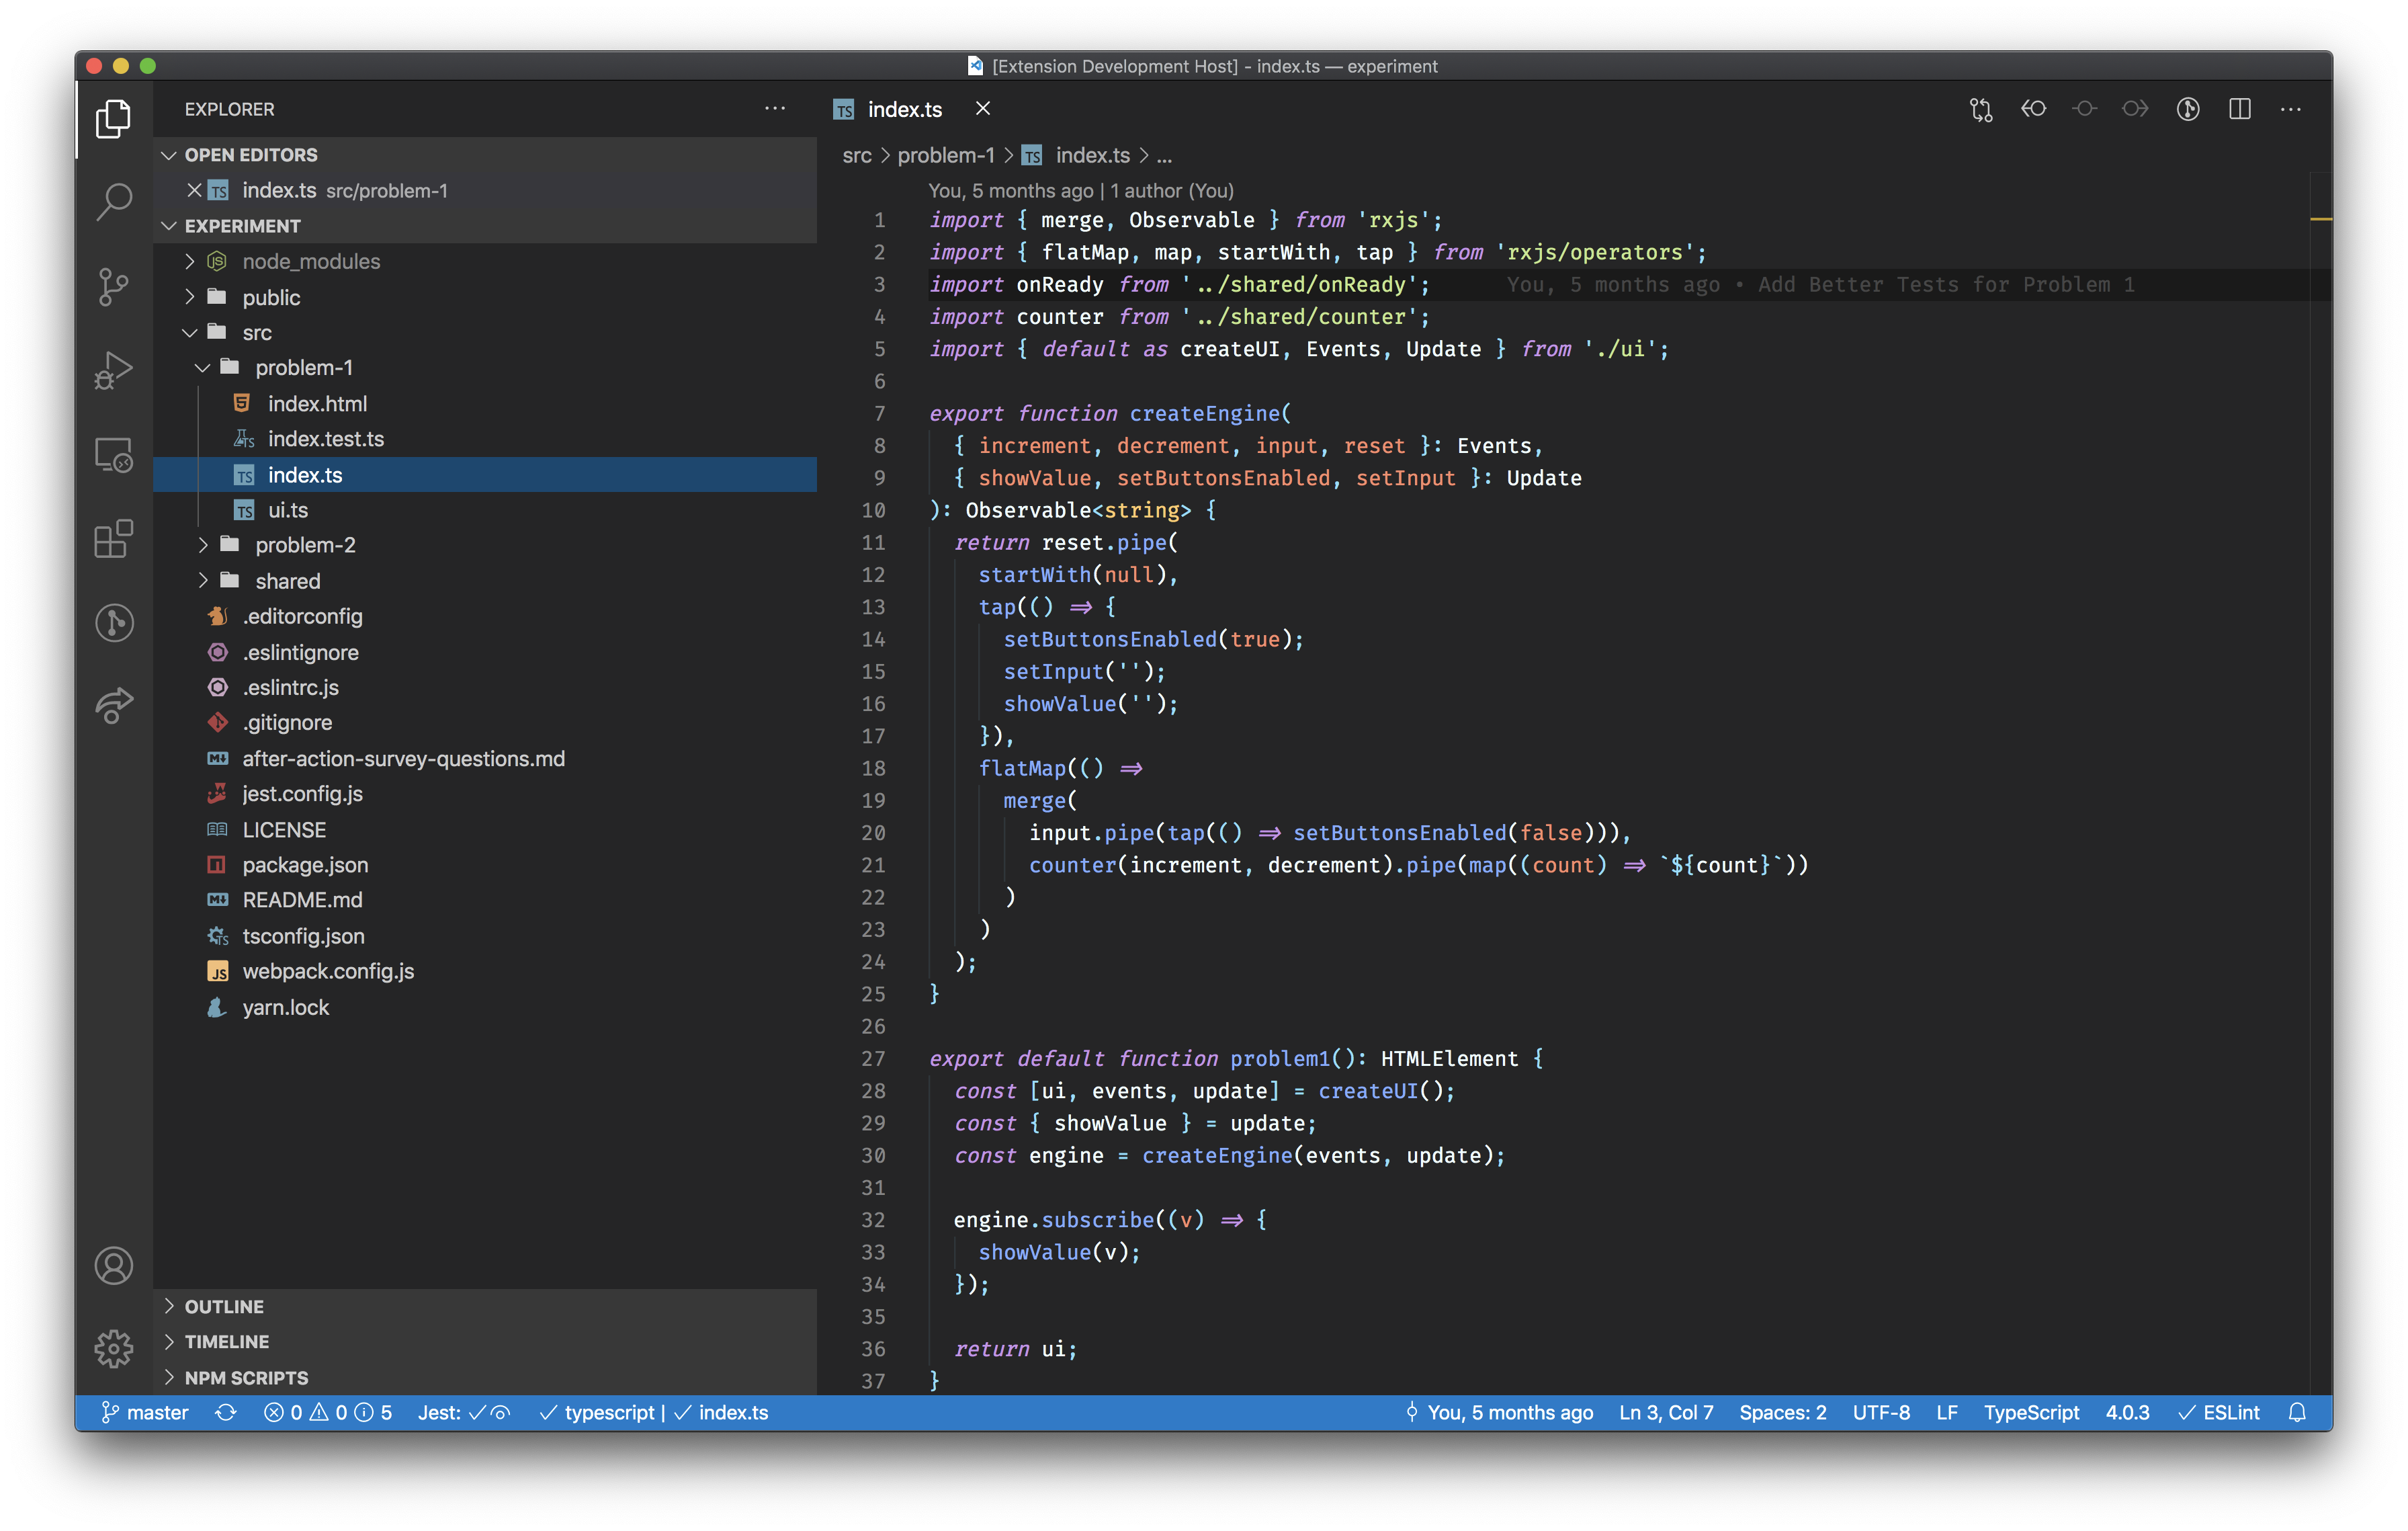
\includegraphics[width=\columnwidth]{walkthrough-screenshots/step1.png}
	\Description{}
	\caption{Visual Studio Code after opening the \texttt{index.ts} file.}
	\label{fig:walkthrough-screesnhot-step-1}
\end{figure}


\subsubsection{Navigate to Operator}
Move cursor the \texttt{flatMap} operator on Line~18.

\begin{itemize}
	\item Visual Studio Code: Shows code actions icon in front of Line~18.
	\item Success story:
	      \begin{itemize}
	      	\item The original task clearly describes the hypothesis regarding this line/piece of source code. Hence, navigating here seems the natural course of action for the user.
	      \end{itemize}
\end{itemize}

\begin{figure}[ht]
	\centering
	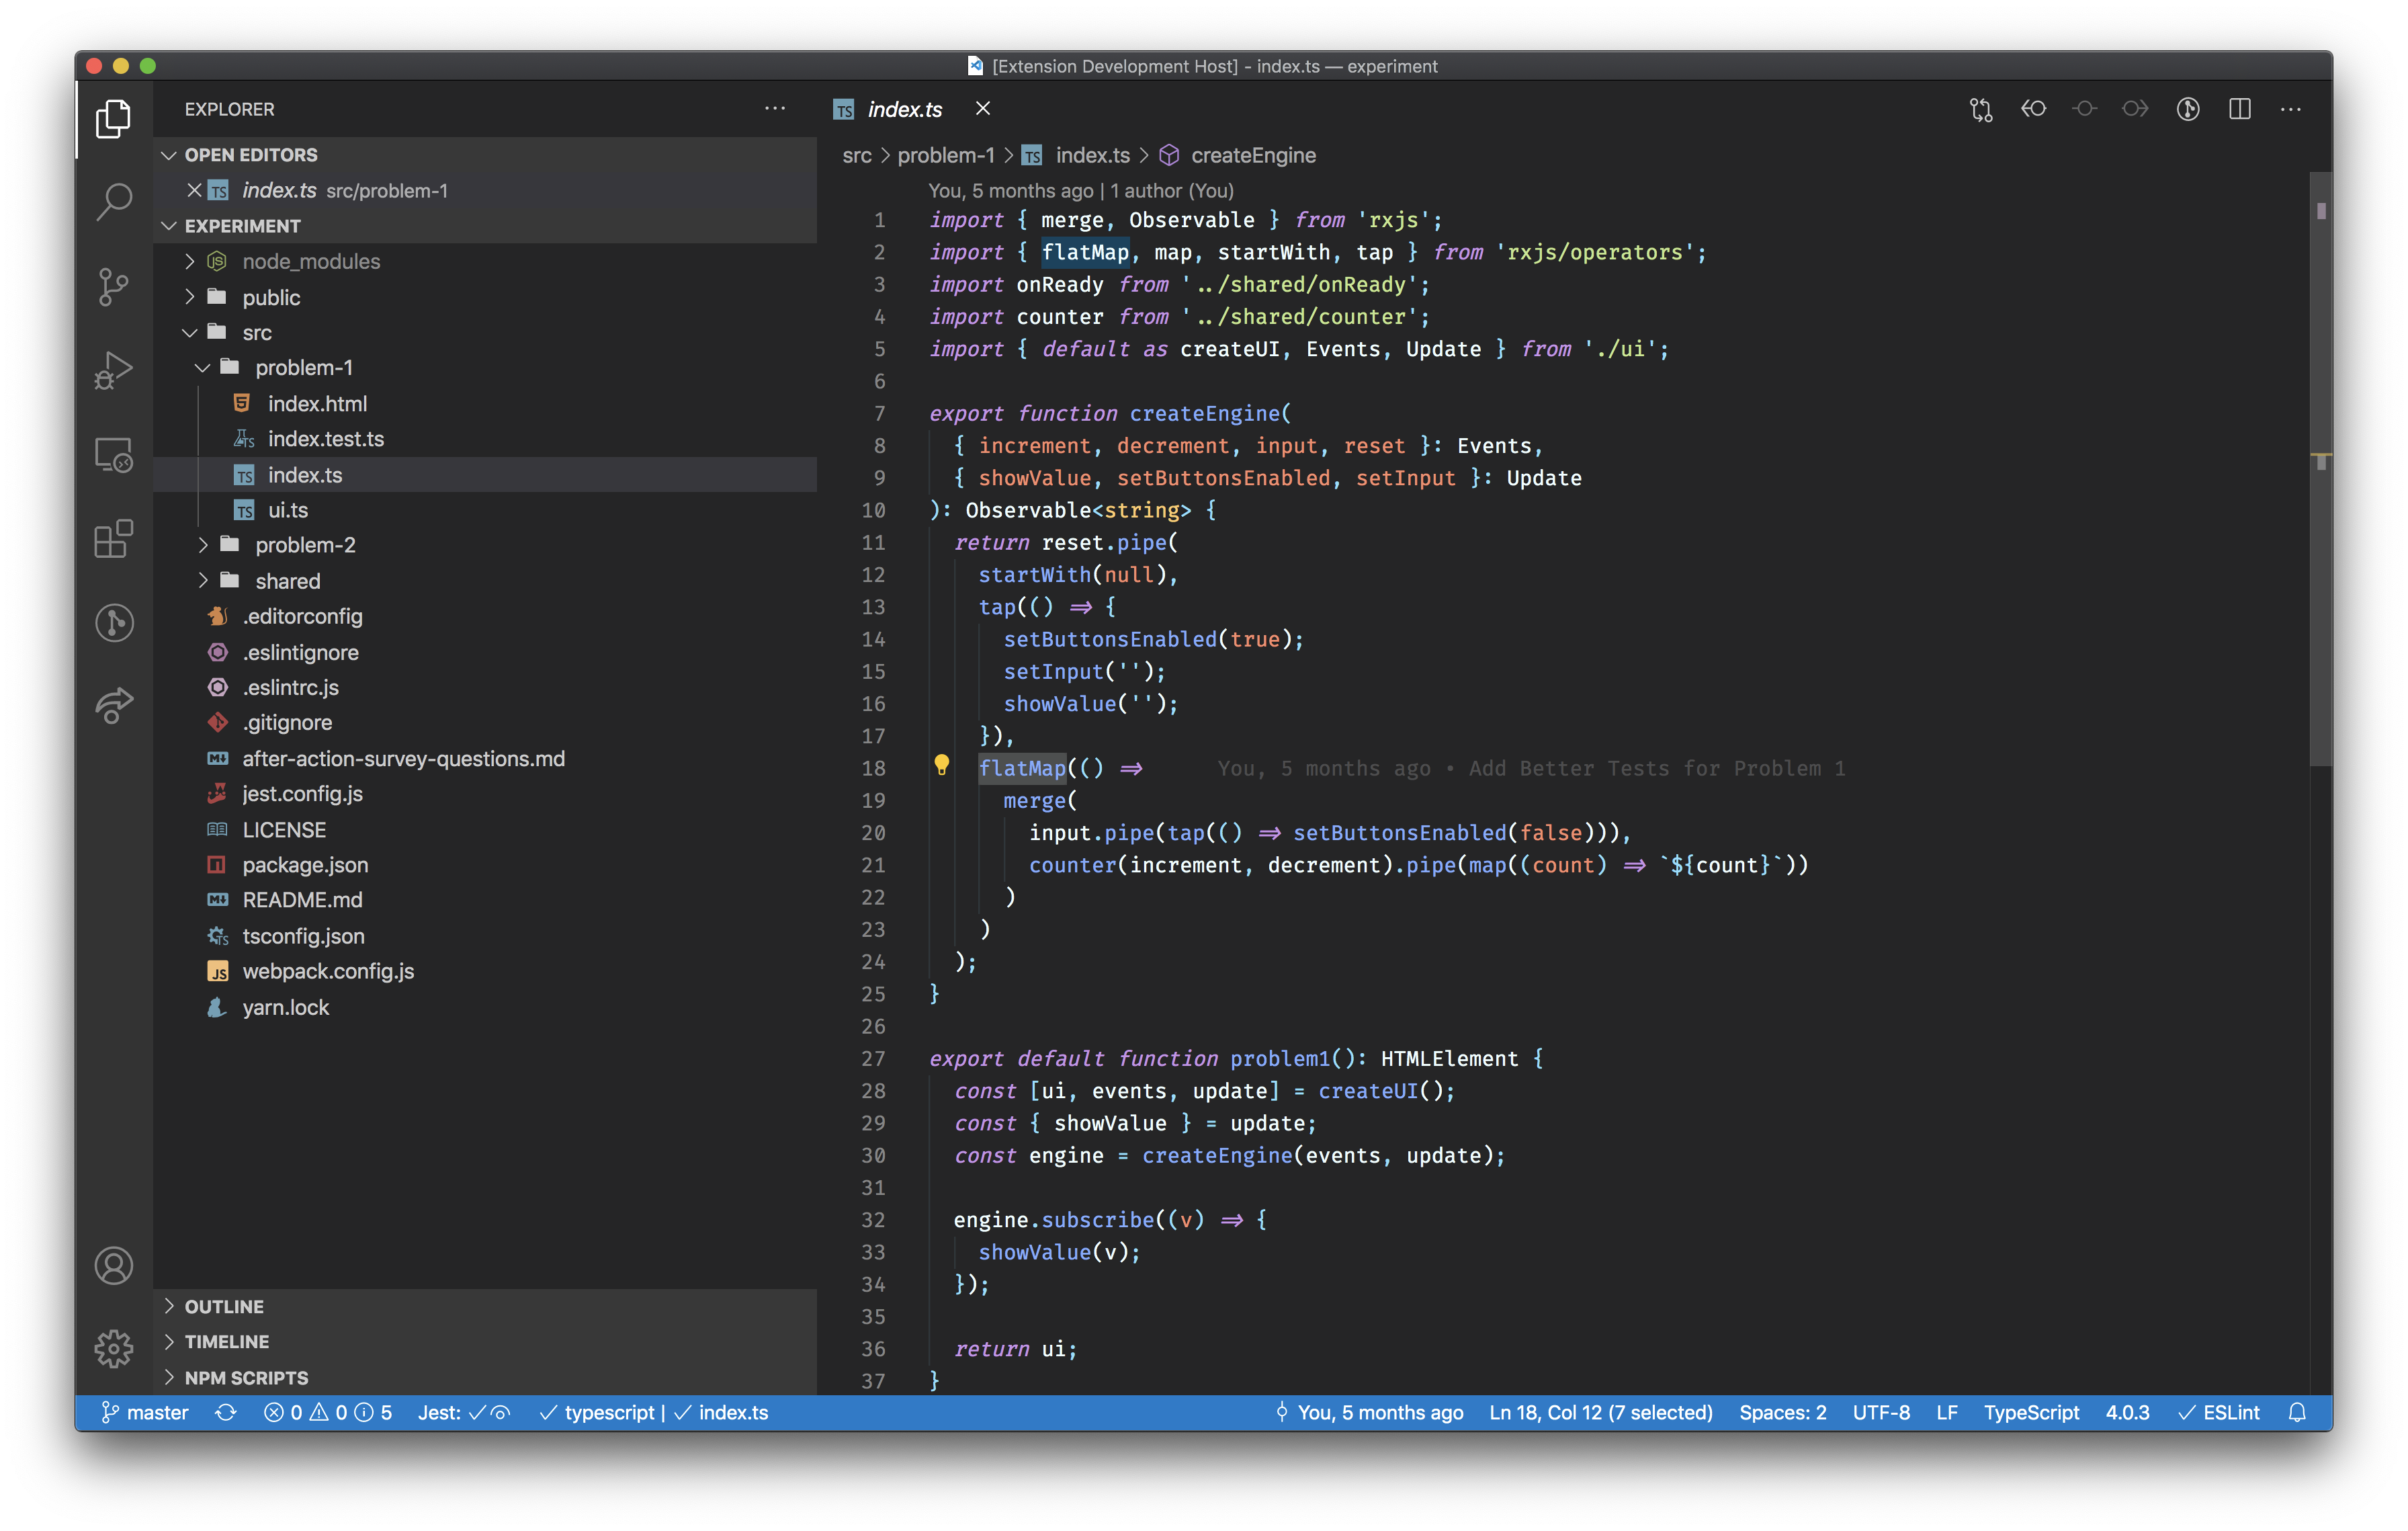
\includegraphics[width=\columnwidth]{walkthrough-screenshots/step2.png}
	\Description{}
	\caption{Visual Studio Code after navigating cursor to the \texttt{flatMap} operator on Line~18.}
	\label{fig:walkthrough-screesnhot-step-2}
\end{figure}


\subsubsection{Open Code Actions}
Open the code actions menu by clicking the yellow light bulb icon.

\begin{itemize}
	\item Visual Studio Code: Shows available code actions.
	\item Failure story:
	      \begin{itemize}
	      	\item Will the user know that the correct action is available?
	      	      \begin{itemize}
	      	      	\item The user might know code actions for providing options to refactor a piece of code or quick fixes for code linting problems. It is questionable if he will expect functionality to inspect parts of a data flow graph here.
	      	      \end{itemize}
	      \end{itemize}
\end{itemize}

\begin{figure}[ht]
	\centering
	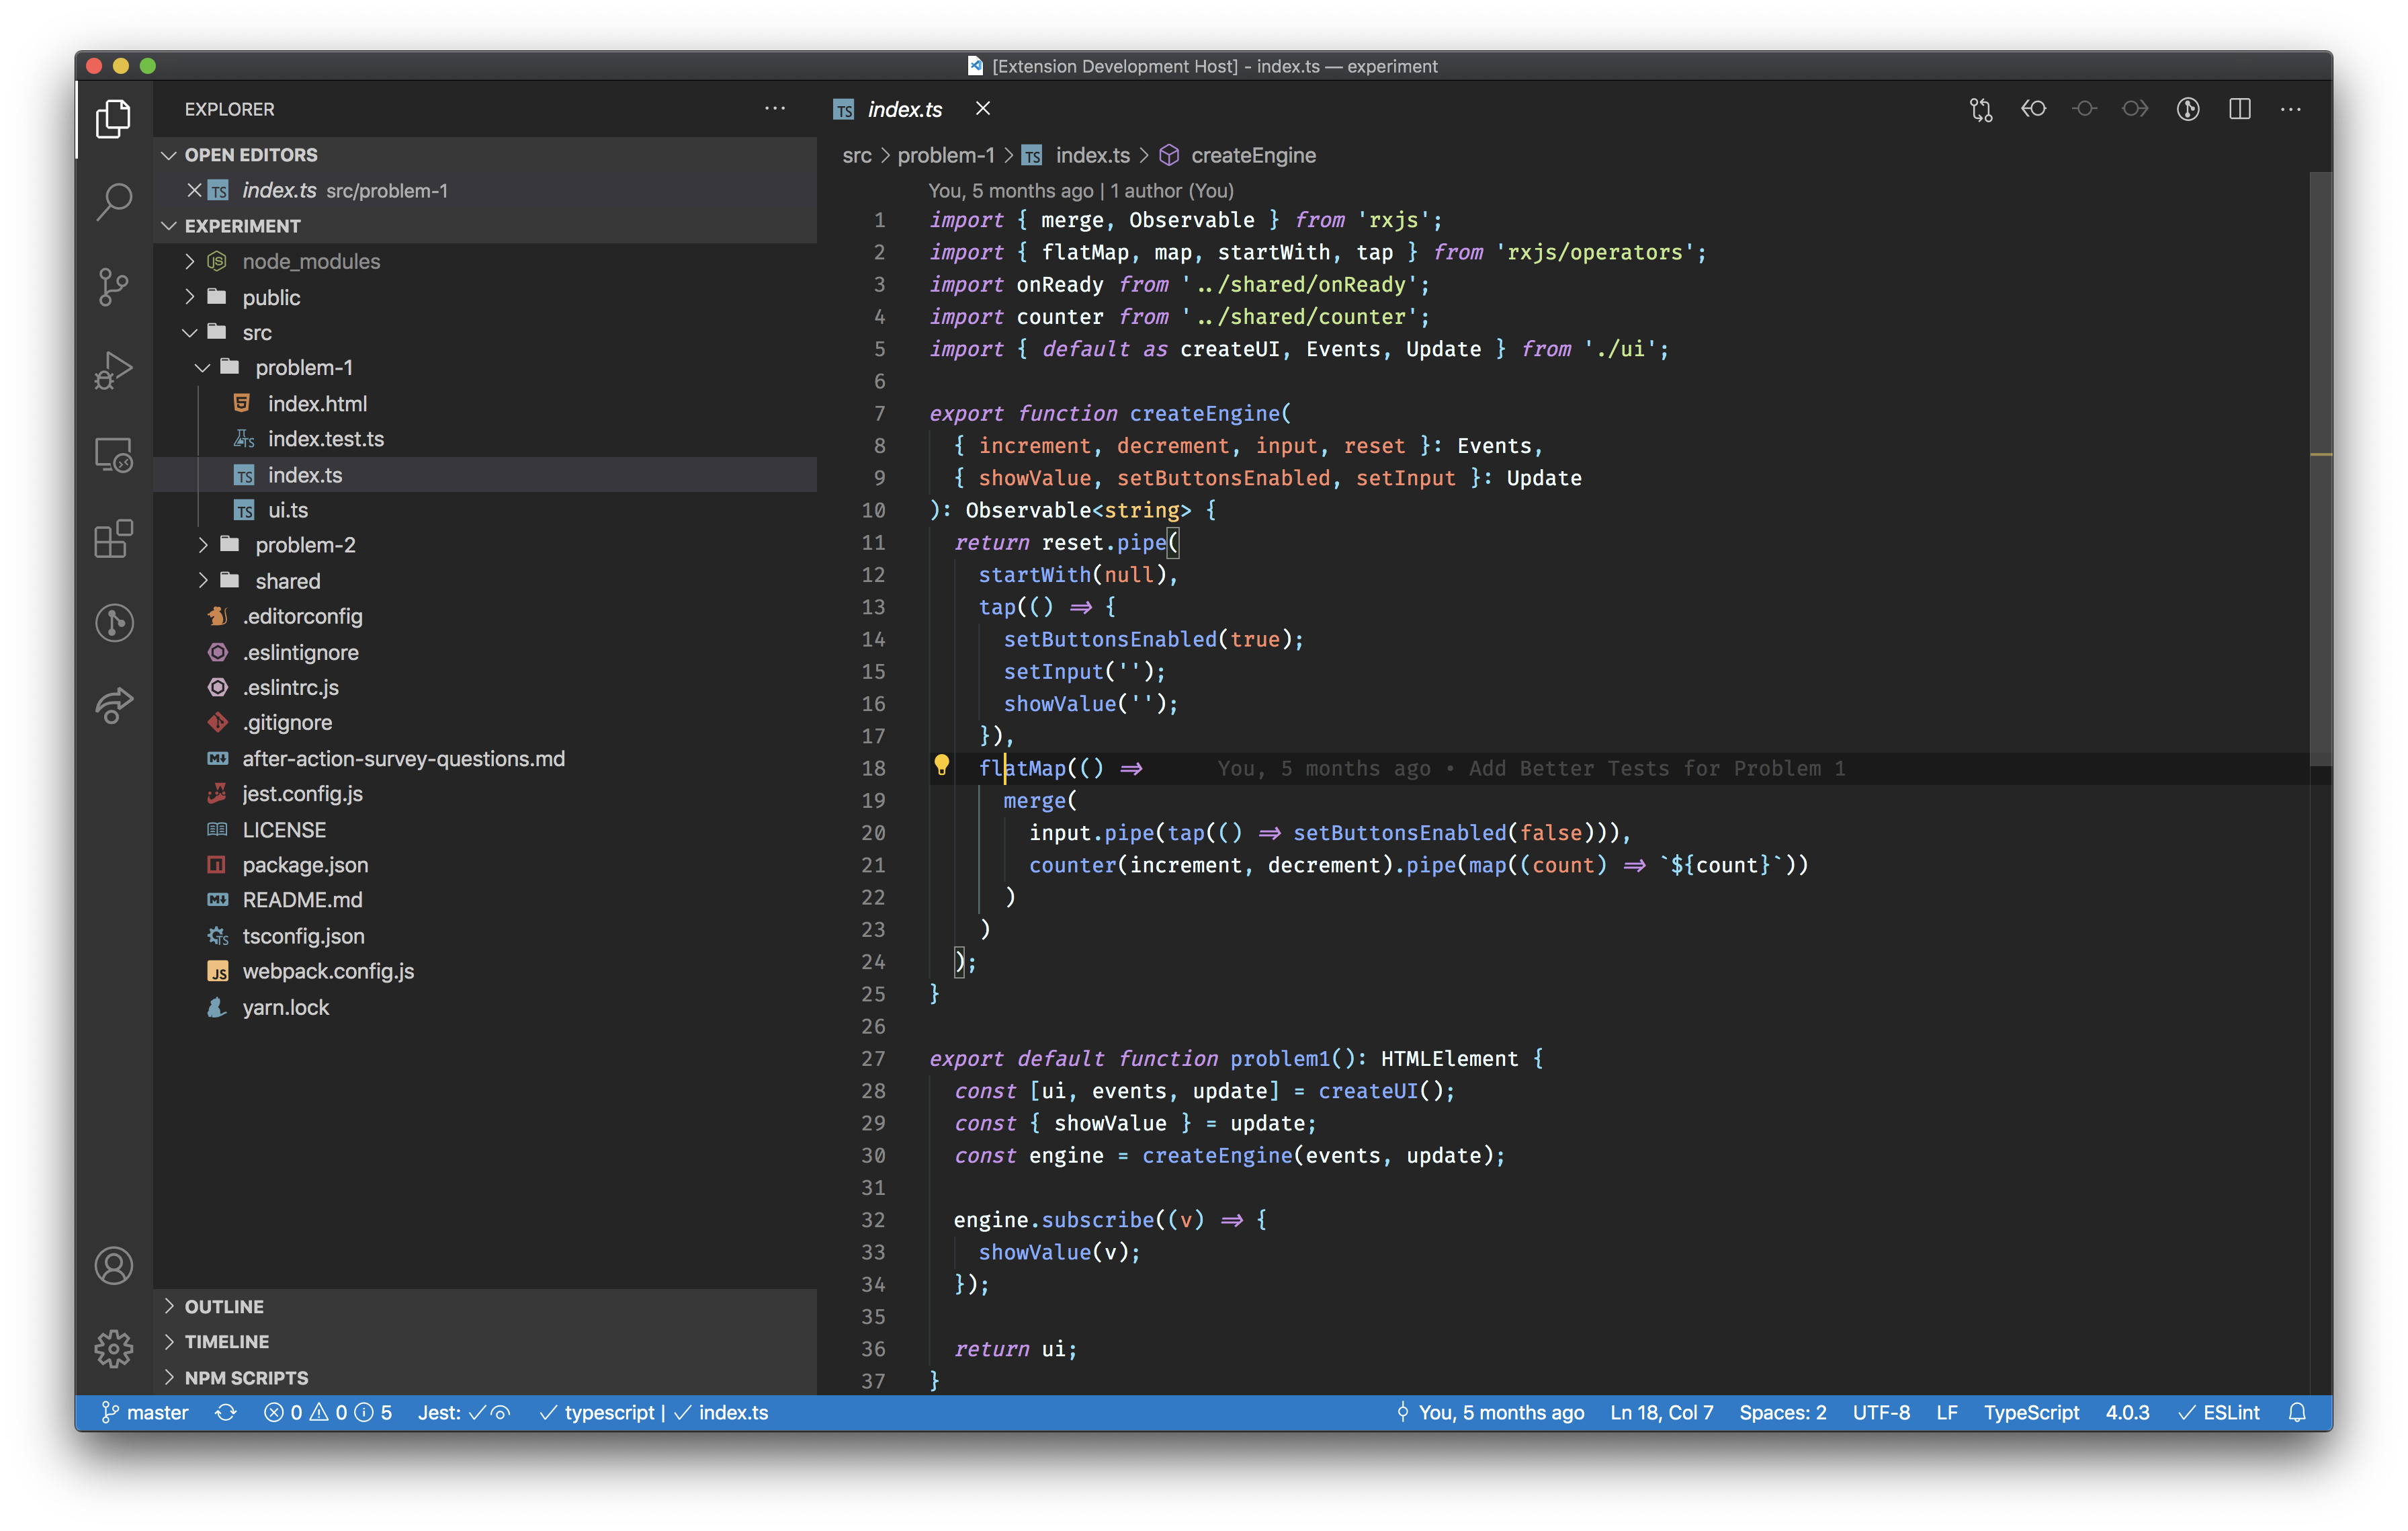
\includegraphics[width=\columnwidth]{walkthrough-screenshots/step3and4.png}
	\Description{}
	\caption{Visual Studio Code indicating available code actions on Line~18 using a yellow light bulb icon.}
	\label{fig:walkthrough-screesnhot-step-3}
\end{figure}


\subsubsection{Create Probe for Operator}
Select ``Probe Observable...'' code action from the related menu.

\begin{itemize}
	\item Visual Studio Code: Adds \texttt{flatMap} operator on Line~18 to "Observables" list in debugging view.
	\item Failure story:
	      \begin{itemize}
	      	\item If the correct action is taken, will the user see that things are going ok?
	      	      \begin{itemize}
	      	      	\item The ``Observables'' list is part of the debugging view of Visual Studio Code. The user will not get any feedback that his action ``Probe Observable...'' was successful without changing the view manually to debugging and expanding the ``Observables'' panel in the lower left.
	      	      \end{itemize}
	      \end{itemize}
\end{itemize}


\subsubsection{Open Observable Probe Monitor}
Open the ``Observable Probe Monitor'' view using command palette.

\begin{itemize}
	\item Visual Studio Code: Shows empty ``Observable Probe Monitor'' view
	\item Failure story:
	      \begin{itemize}
	      	\item Will the user know that the correct action is available?
	      	      \begin{itemize}
	      	      	\item The user might not be aware that the ``Observable Probe Monitor'' view is hidden within the command palette. Hence, they might feel lost after adding the observable probe in the previous step.
	      	      \end{itemize}
	      	\item If the correct action is taken, will the user see that things are going ok?
	      	      \begin{itemize}
	      	      	\item The user might get confused by the ``Observable Probe Monitor'' being blank by default.
	      	      \end{itemize}
	      \end{itemize}
\end{itemize}

\begin{figure}[ht]
	\centering
	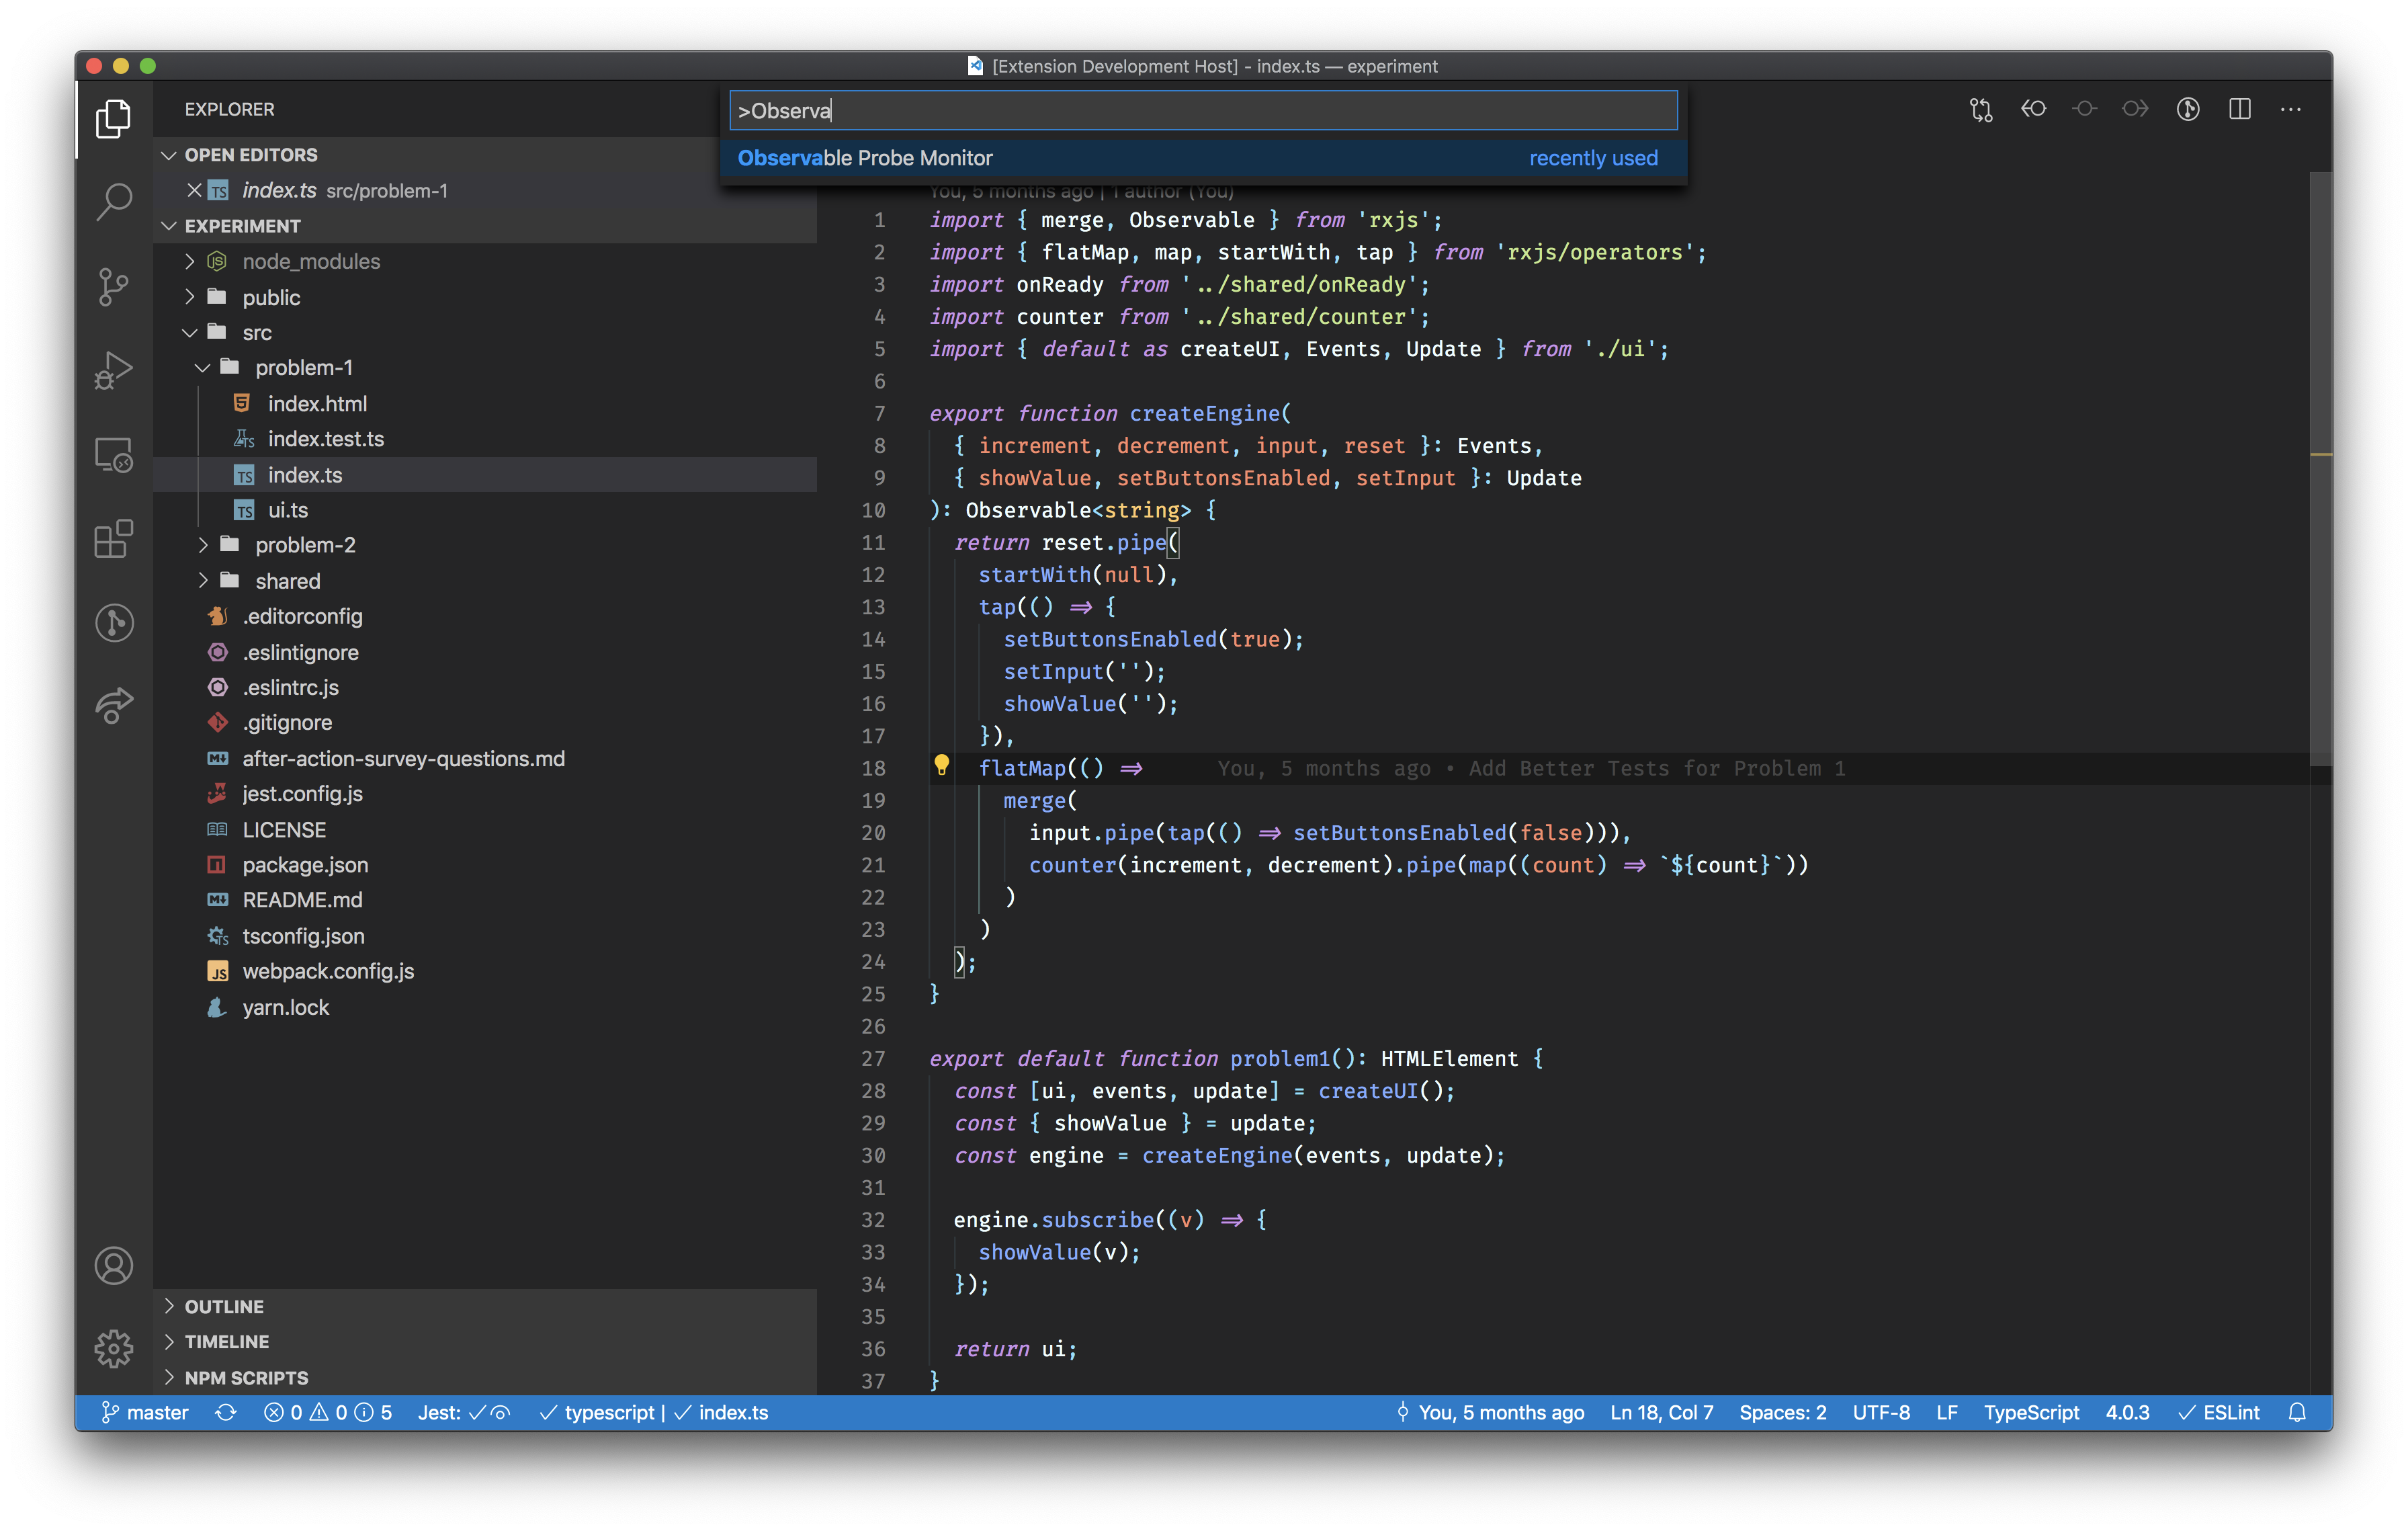
\includegraphics[width=\columnwidth]{walkthrough-screenshots/step5-1.png}
	\Description{}
	\caption{Visual Studio Codes command palette menu showing the ``Observable Probe Monitor'' command.}
	\label{fig:walkthrough-screesnhot-step-5-1}
\end{figure}

\begin{figure}[ht]
	\centering
	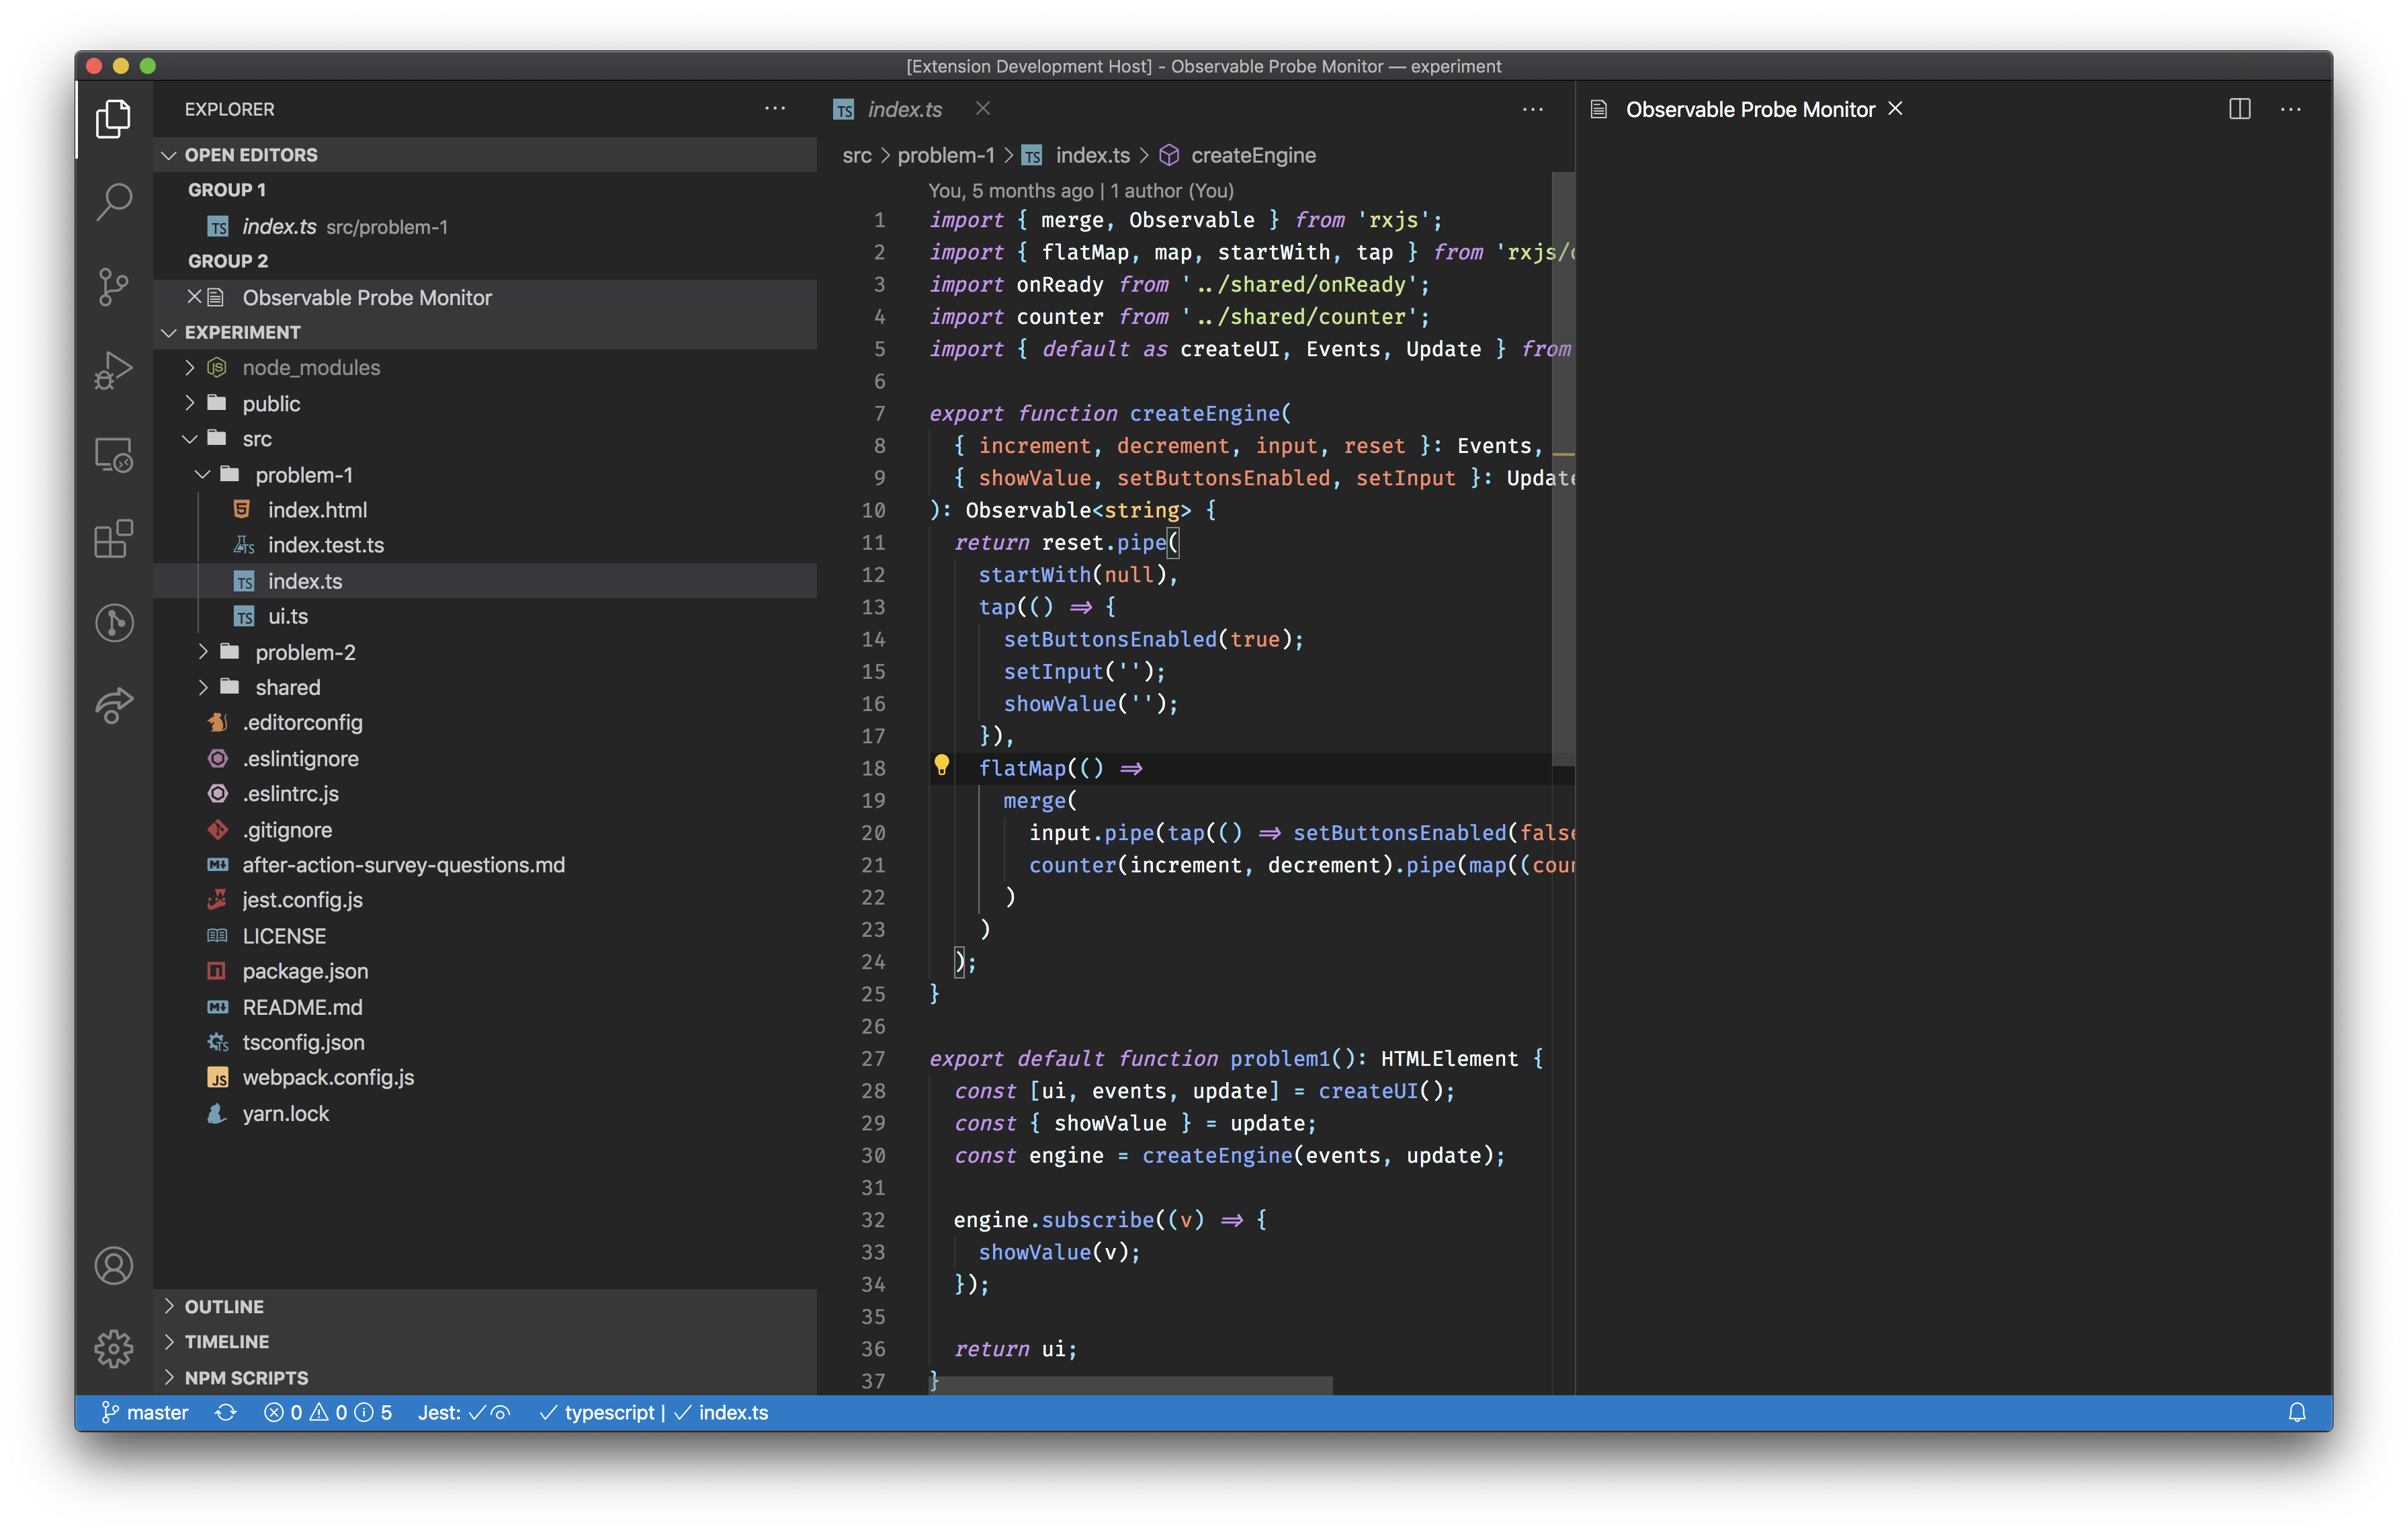
\includegraphics[width=\columnwidth]{walkthrough-screenshots/step5-2.png}
	\Description{}
	\caption{Visual Studio Code showing the empty Observable Probe Monitor on the right pane.}
	\label{fig:walkthrough-screesnhot-step-5-2}
\end{figure}

\subsubsection{Launch Application}
Execute ``Problem~1'' launch configuration

\begin{itemize}
	\item Visual Studio Code: Opens default browser showing ``Problem~1''
	\item Default Browser: Shows ``Problem~1'' UI
	\item Success story:
	      \begin{itemize}
	      	\item The users previous experience with Visual Studio Code launch configuration allows assuming this the natural course of action in order to prepare himself for further inspection of the application.
	      \end{itemize}
\end{itemize}

\begin{figure}[ht]
	\centering
	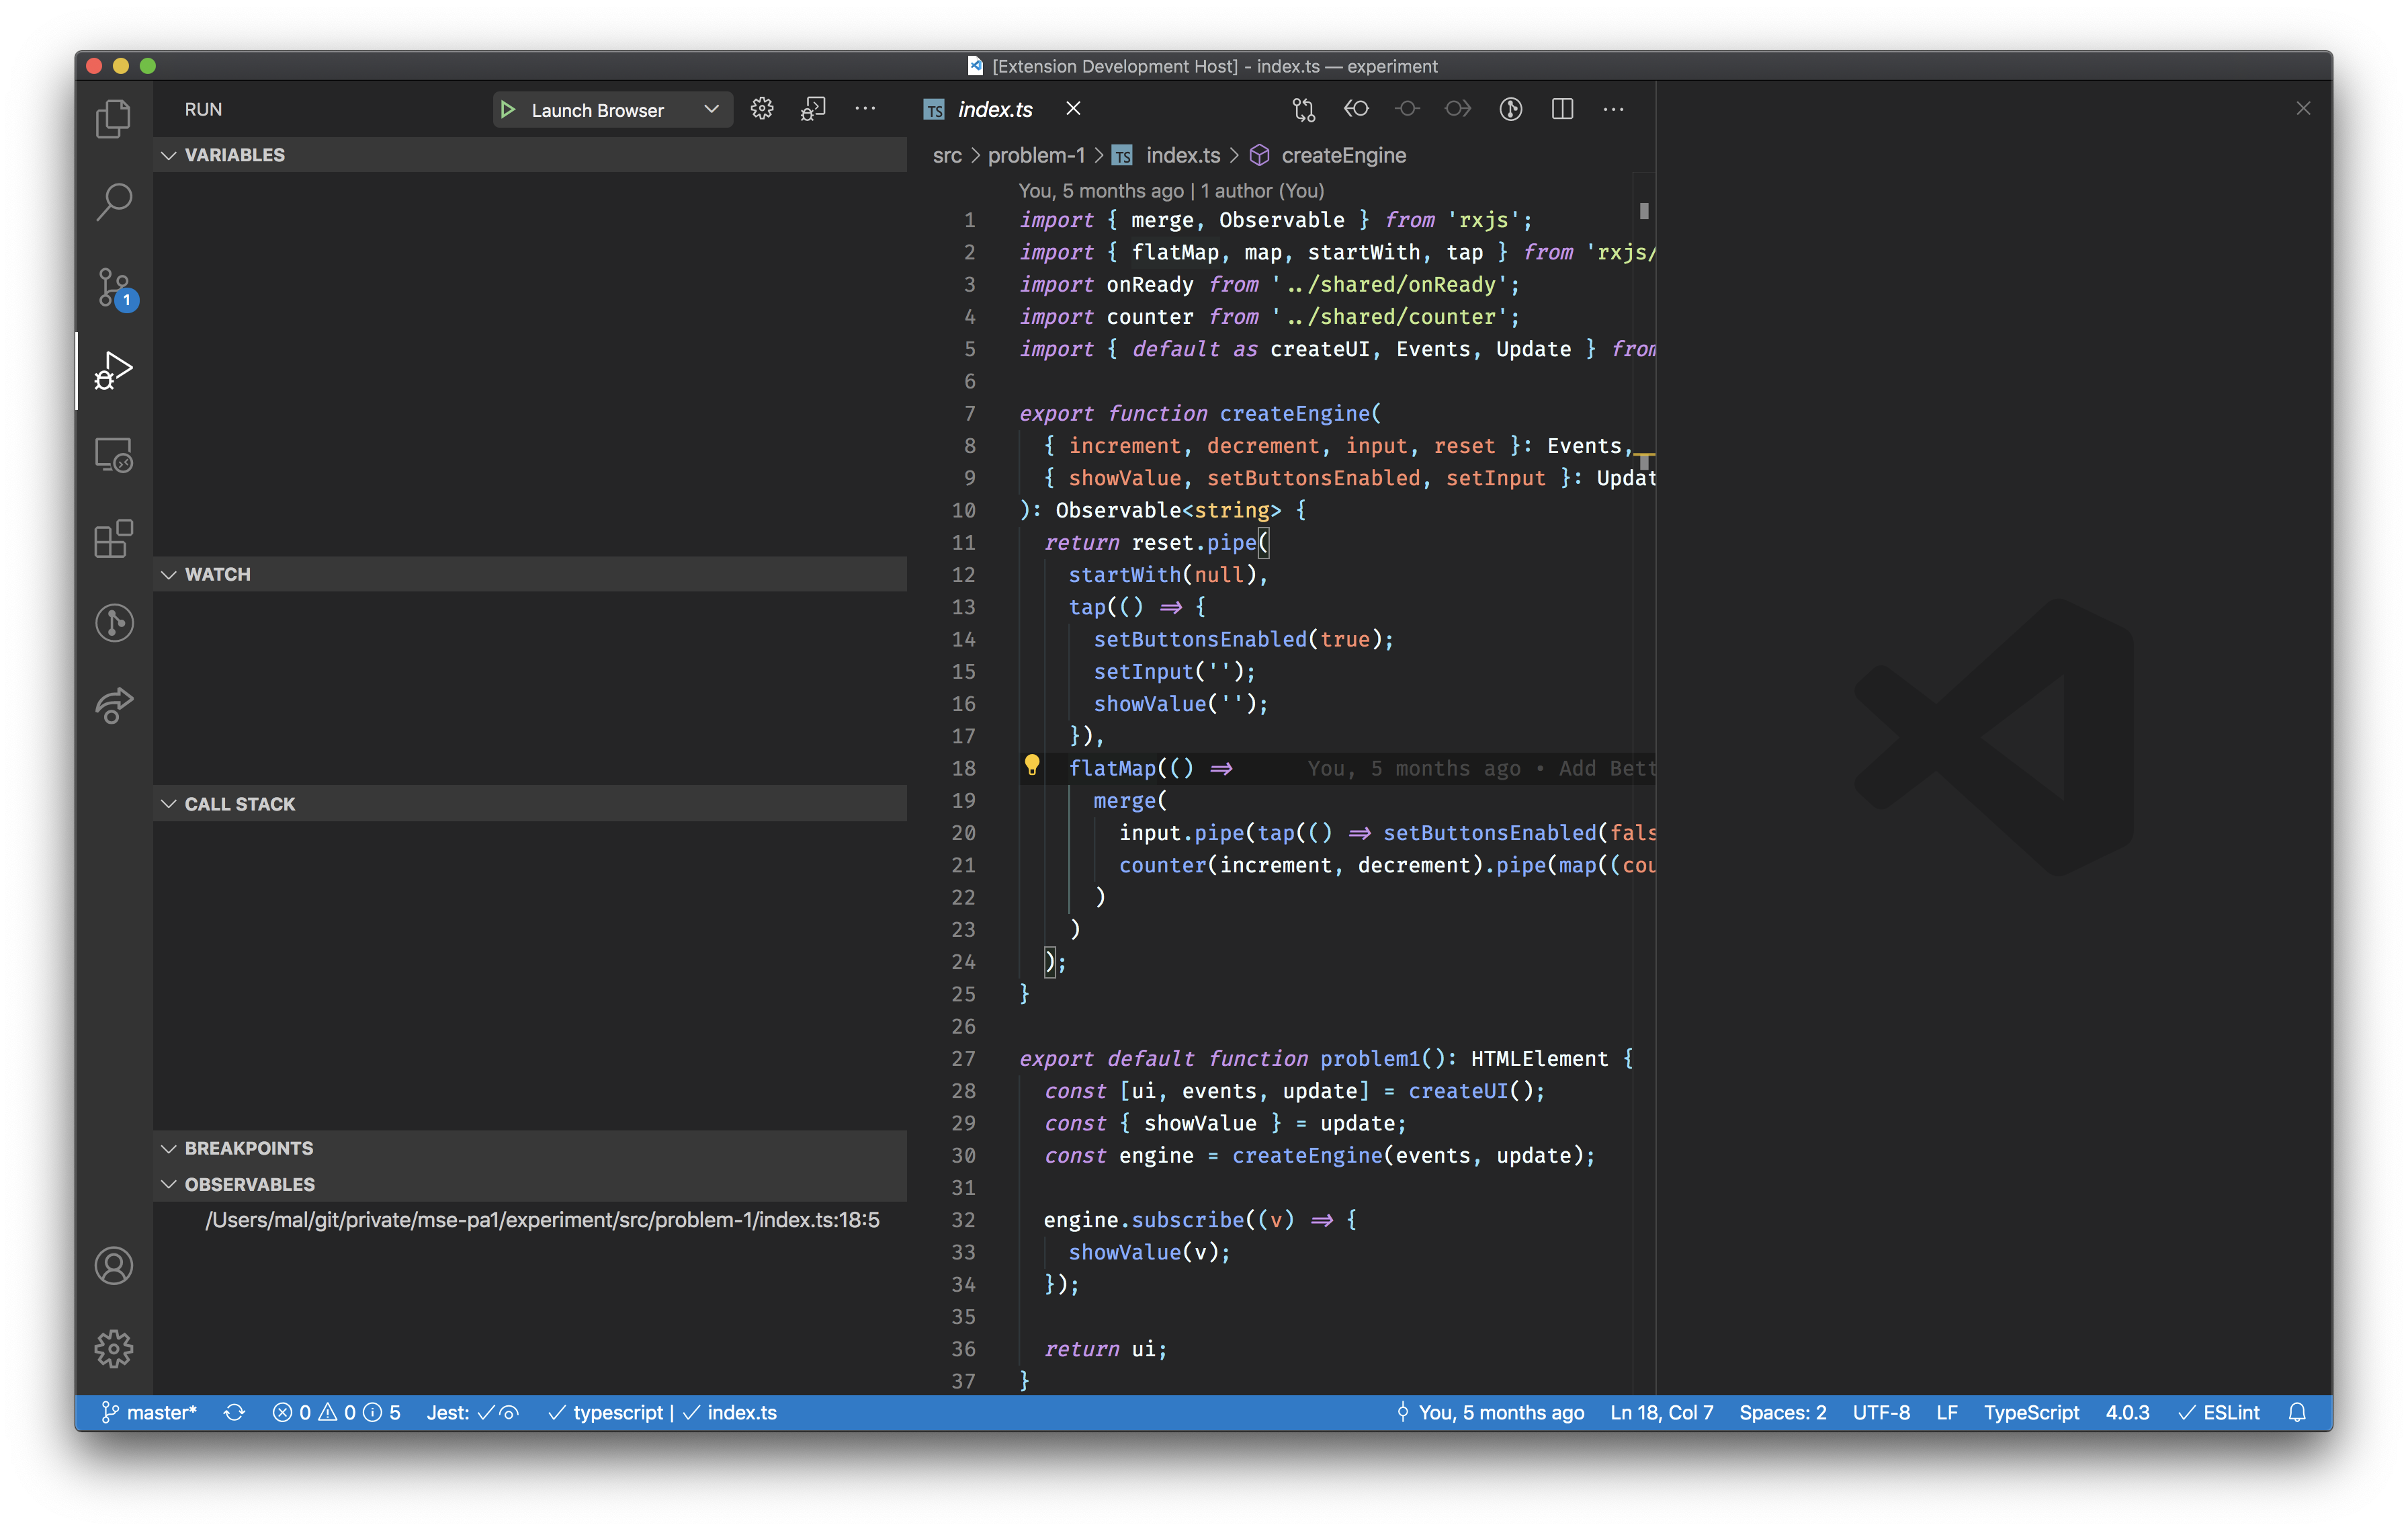
\includegraphics[width=\columnwidth]{walkthrough-screenshots/step6.png}
	\Description{}
	\caption{Visual Studio Code showing the debugging view after launching ``Problem~1''.}
	\label{fig:walkthrough-screesnhot-step-6}
\end{figure}

\subsubsection{Interact with Application}
Interact with ``Problem~1'' in the default browser.

\begin{itemize}
	\item Visual Studio Code: ``Observable Probe Monitor'' provides live telemetry information about values and life cycle events produced by the \texttt{flatMap} operator.
	\item Failure story:
	      \begin{itemize}
	      	\item Will the user know that the correct action will achieve the desired effect?
	      	      \begin{itemize}
	      	      	\item The user might not be aware that he is expected to interact with ``Problem~1'' in the default browser in order to get live feedback in the ``Observable Probe Monitor''.
	      	      \end{itemize}
	      	\item If the correct action is taken, will the user see that things are going ok?
	      	      \begin{itemize}
	      	      	\item The default browser might overlay Visual Studio Code and the ``Observable Probe Monitor'' view. This is why the user might miss the live trace of values and life cycle events displayed in the ``Observable Probe Monitor''.
	      	      \end{itemize}
	      \end{itemize}
\end{itemize}

\begin{figure}[ht]
	\centering
	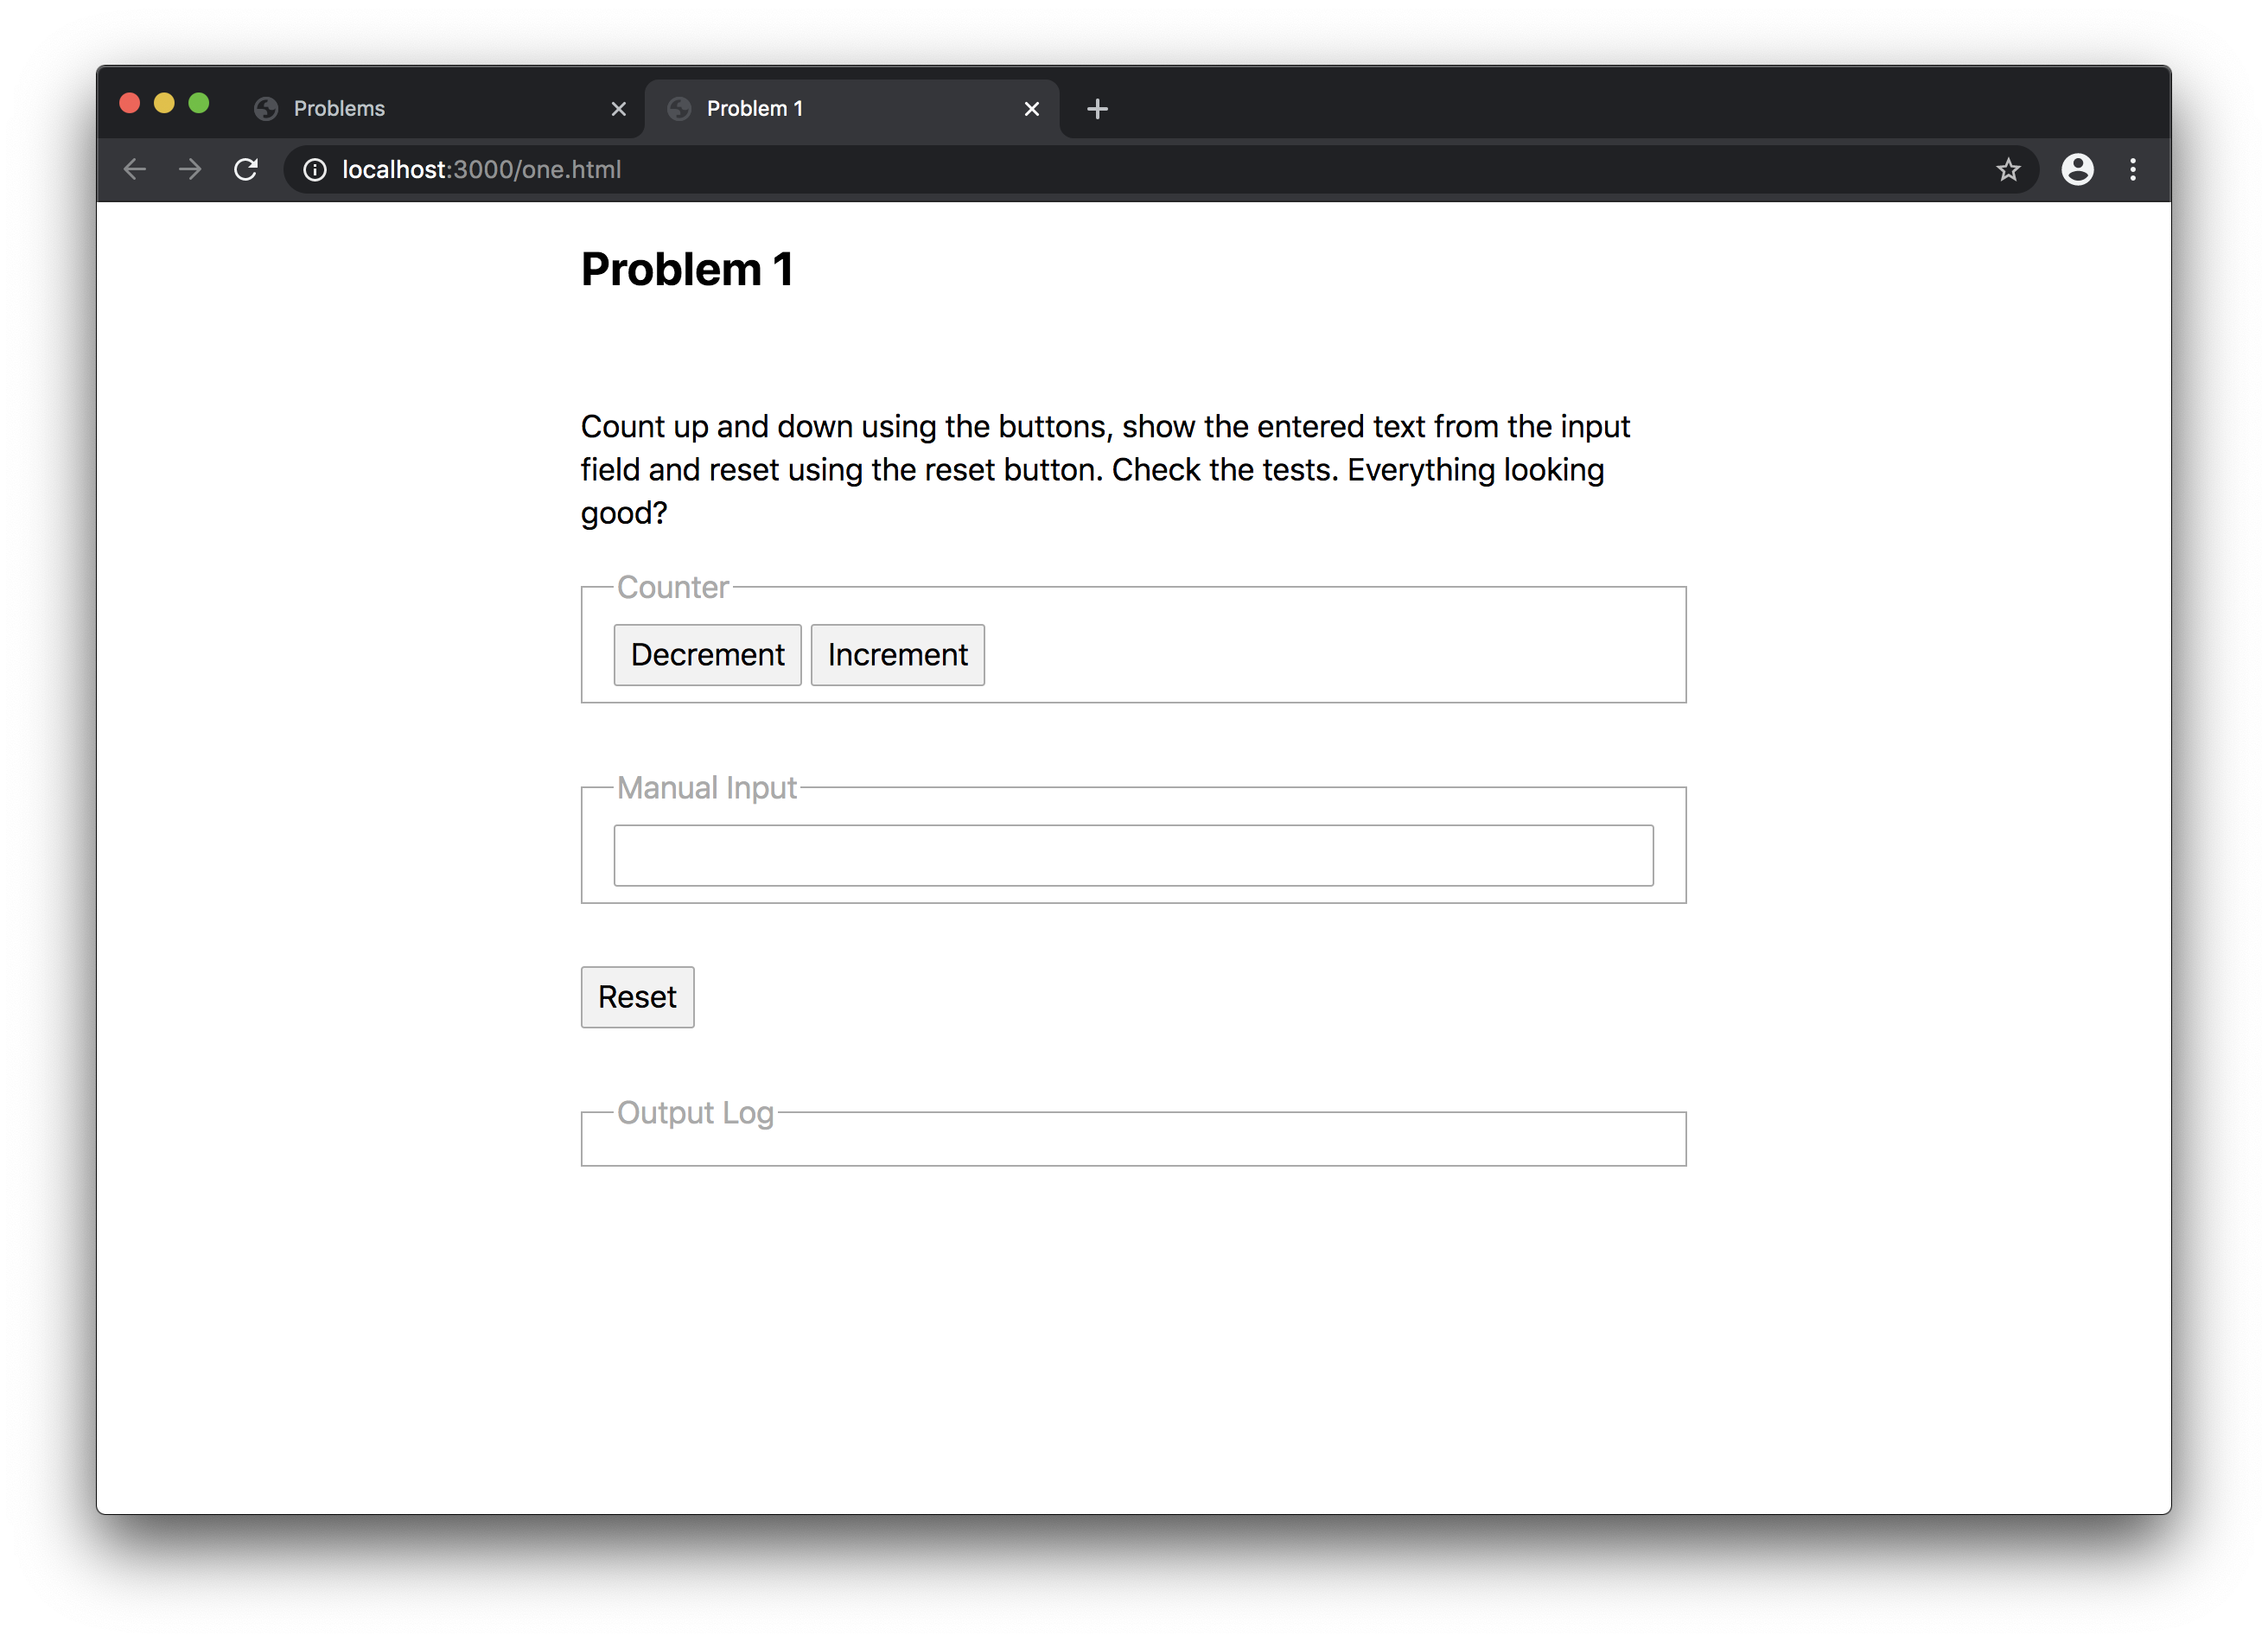
\includegraphics[width=\columnwidth]{walkthrough-screenshots/step7.png}
	\Description{}
	\caption{Google Chrome displaying the user interface of ``Problem~1'' ready to receive interactions.}
	\label{fig:walkthrough-screesnhot-step-7}
\end{figure}

\subsubsection{Interpret Runtime Behavior}
Interpret the live trace of emitted values and life cycle events in the ``Observable Probe Monitor'' view

\begin{itemize}
	\item Visual Studio Code: Provides detail information to a traced item
	\item Success story:
	      \begin{itemize}
	      	\item The original task states that the user is interested in more close information regarding the \texttt{flatMap} operator. Since the ``Observable Probe Monitor'' provide such information in real-time, we can expect the user to use this information accordingly.
	      \end{itemize}
\end{itemize}

\begin{figure}[ht]
	\centering
	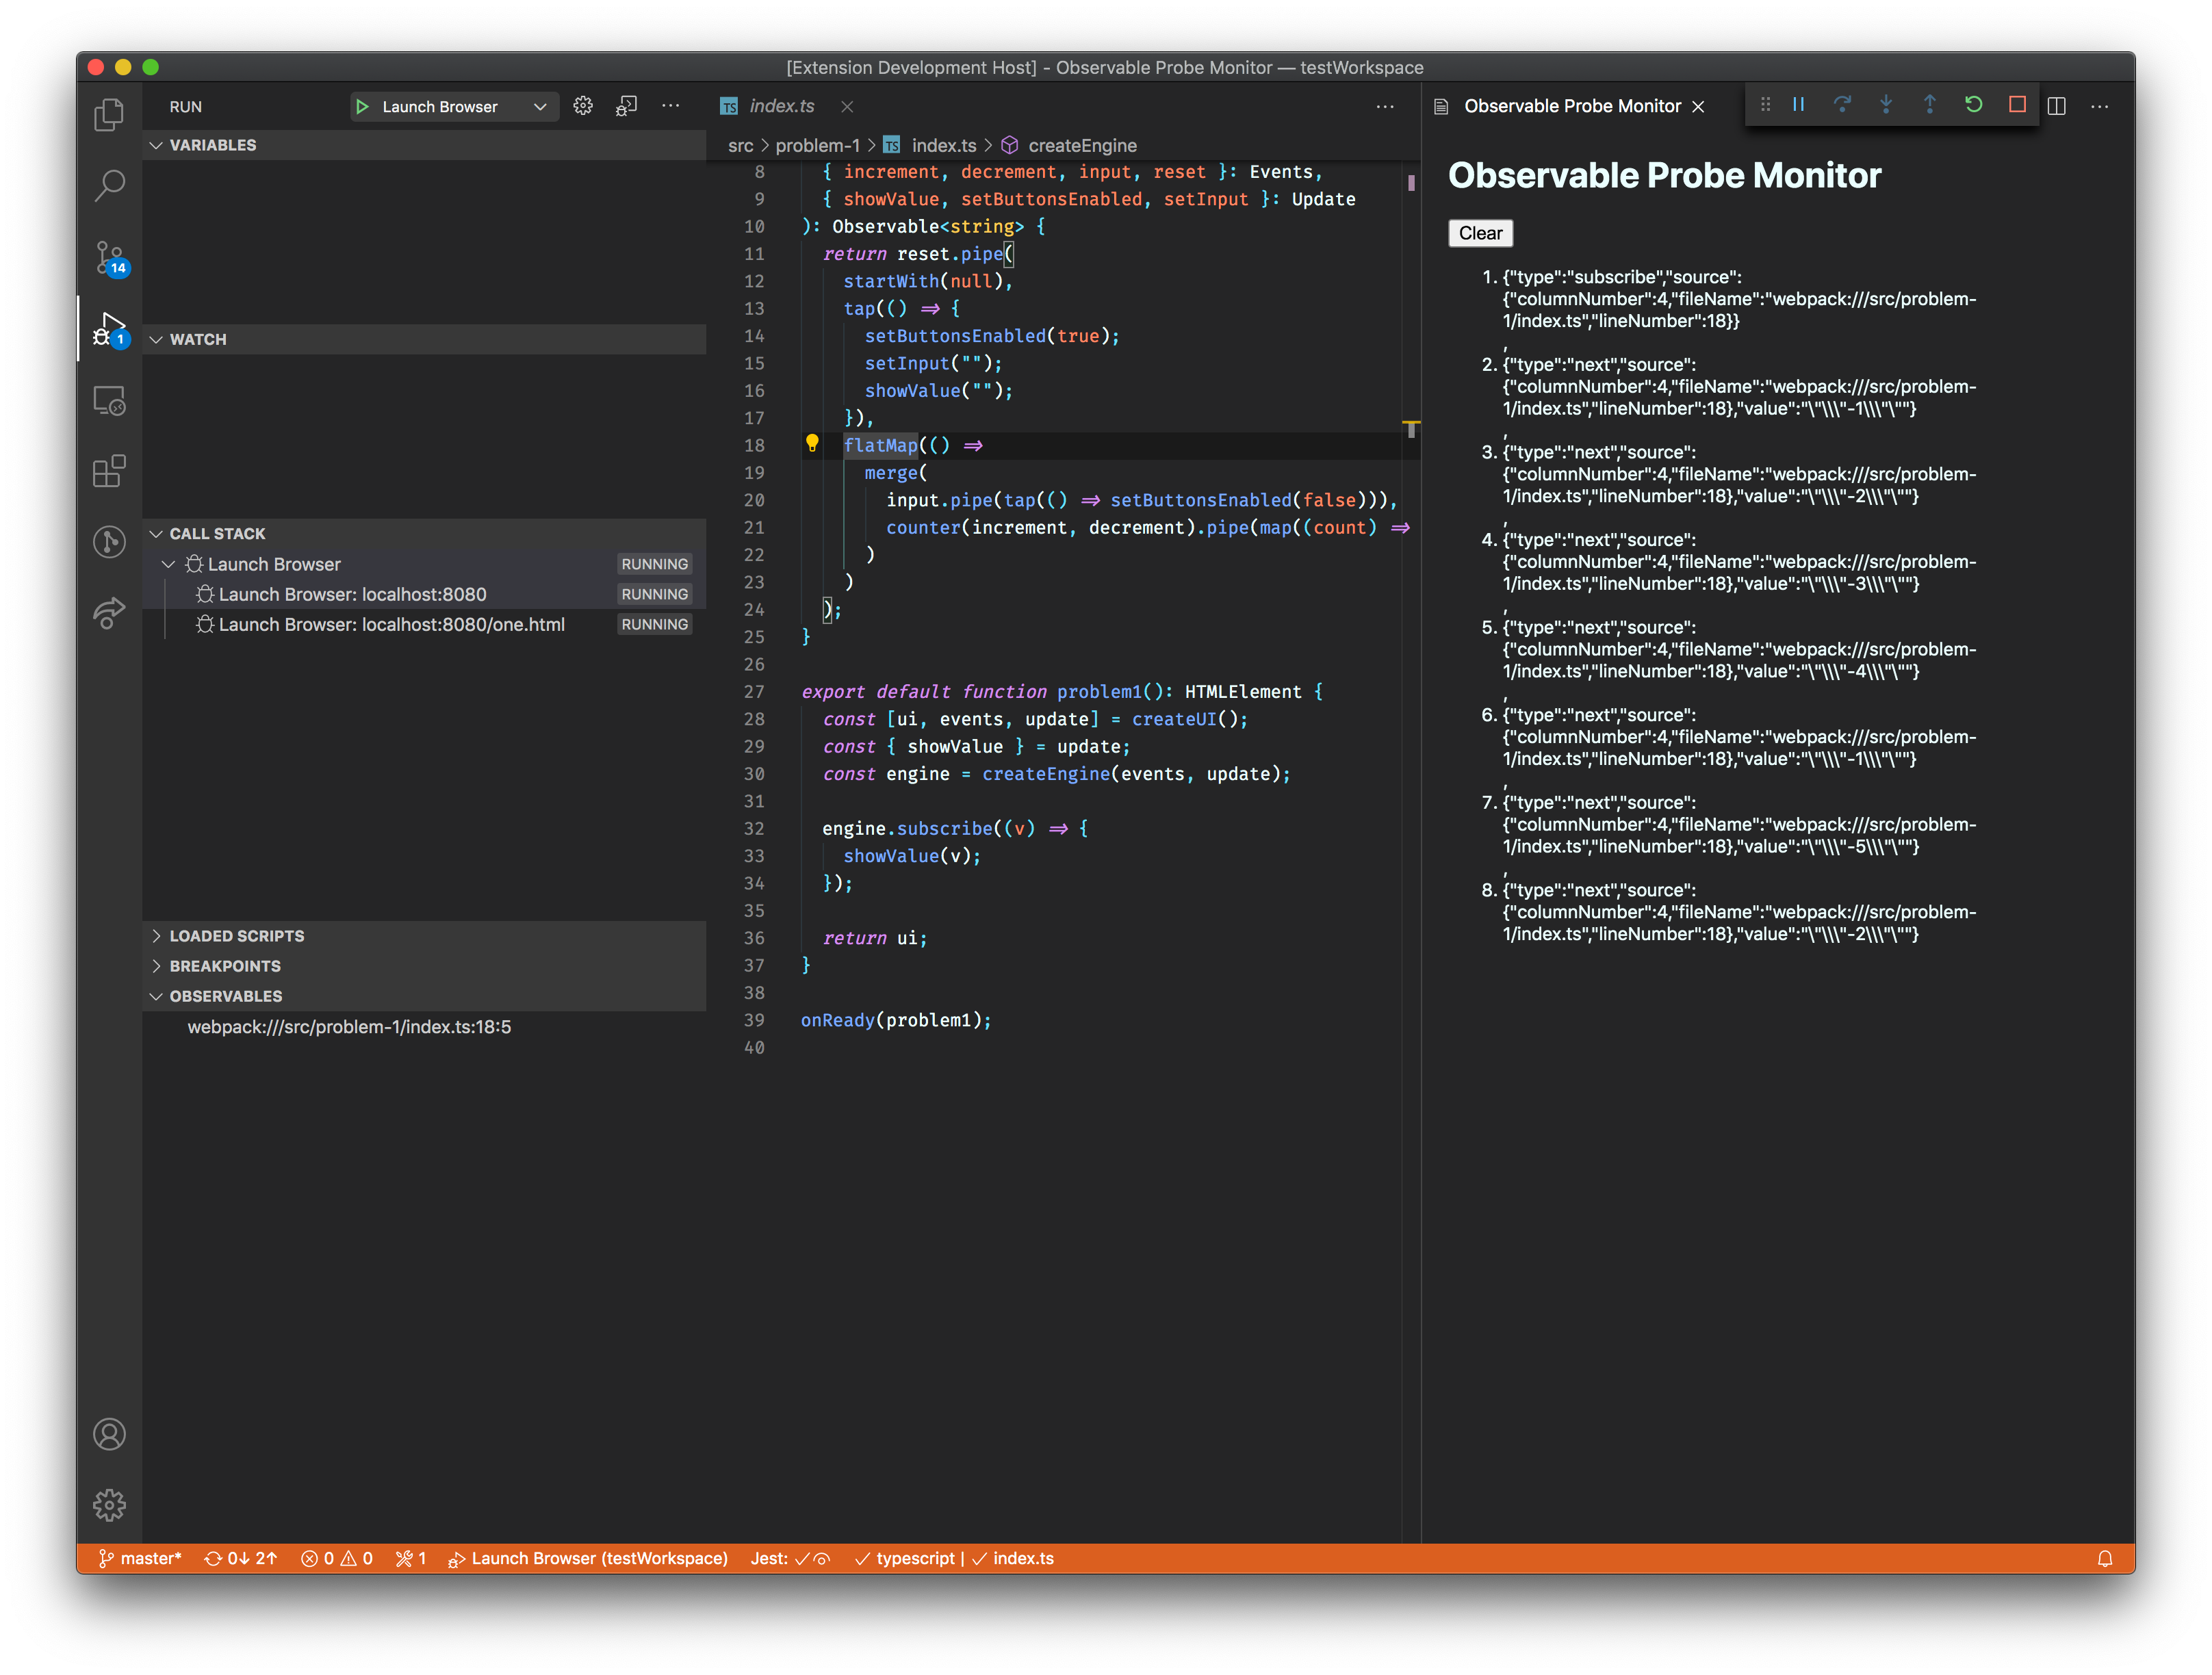
\includegraphics[width=\columnwidth]{walkthrough-screenshots/step8.png}
	\Description{}
	\caption{Visual Studio Code showing live telemetry in the ``Observable Probe Monitor''.}
	\label{fig:walkthrough-screesnhot-step-8}
\end{figure}

\end{document}